\chapter{Infrastructure Attacks}
\label{ch:rdma}

Security proofs reason about an idealized machine: one that computes in constant time, emits nothing an observer can measure, and moves bytes over a channel that reveals only their ciphertext. Real deployments run on a physical substrate that violates every one of those assumptions. Transistors consume power as they switch, processors take data-dependent time, and packets traverse a shared fabric whose routing and timing are visible to anyone positioned to watch. Where the preceding parts trusted this substrate to faithfully carry the quantum and post-quantum mechanisms built on top of it, Part~\ref{part:infra} makes the substrate itself the object of study, at the scale of the whole datacenter. This chapter opens that shift on the offensive: it treats the substrate not as a neutral medium but as an attack surface, escalating from the device-level behaviour of individual chips to the datacenter-scale behaviour of the fabric that connects them.

\section{Hardware and Node-Level Infrastructure}
\label{sec:node-infra}

The lowest layer of the physical substrate---the individual silicon chips and local hardware components---presents the most fundamental attack surface. At this node level, the physical and structural behaviour of the hardware exposes secret state directly to co-located or physically proximate adversaries.

\subsection{Passive Side Channels}
\label{sec:passive-side-channels}

Early demonstrations of physical vulnerability focused on \emph{side channels}, a framing that carries an implicit assumption: that the adversary is a passive observer who reads whatever the substrate happens to leak. In the context of infrastructure attacks, classic side channels are a passive, single-chip special case.

The Advanced Encryption Standard (AES) provides a well-known demonstration. While mathematically unbroken, early implementations were famously defeated by differential power analysis (DPA)~\cite{kocher1999differential}. DPA exploits the fact that the power consumed by a processor depends on the data it is processing. By measuring the power drawn while the device encrypts many known plaintexts, an attacker can statistically correlate the physical traces with hypotheses about the secret key. The correct guess produces a pronounced statistical spike, while incorrect ones vanish into noise.

This allows an attacker to recover the secret key one byte at a time. Instead of an exhaustive search that grows exponentially with the key length, the attack breaks the problem into independent, byte-sized guesses. As illustrated in Figure~\ref{fig:dpa}, an unprotected AES-128 implementation on a commodity microcontroller yields its complete 16-byte key through a sequence of trivial single-byte attacks~\cite{lo2016power}. The mathematics is untouched; the physical implementation simply hands the key over.

% Figs reprinted from Lo et al. (2016) under Taylor & Francis thesis-use permission
% (single excerpt, up to 3 figures/tables). Required acknowledgement is in the caption.
\begin{figure}[htbp]
  \centering
  \begin{subfigure}{0.49\linewidth}
    \centering
    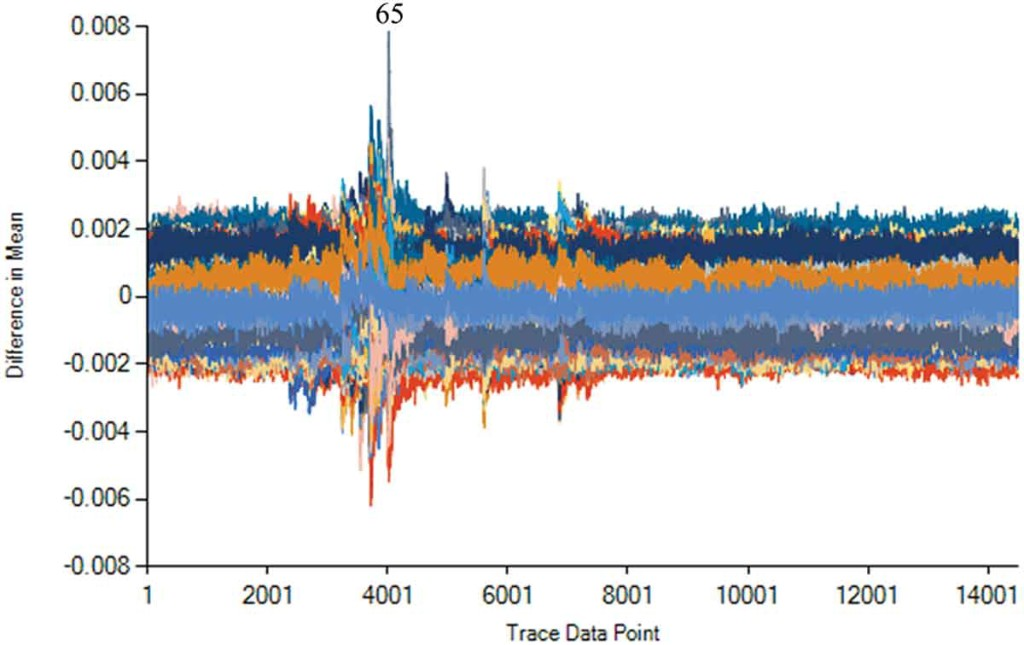
\includegraphics[width=\linewidth]{figures/chapter7/dpa_1byte.png}
    \caption{Recovering a single key byte.}
    \label{fig:dpa-1byte}
  \end{subfigure}
  \hfill
  \begin{subfigure}{0.49\linewidth}
    \centering
    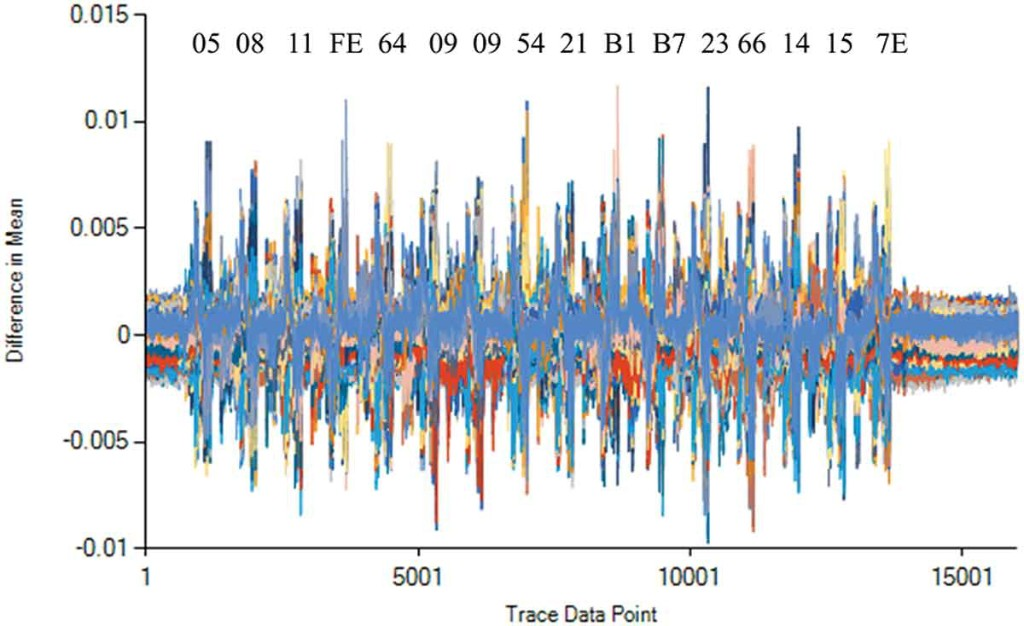
\includegraphics[width=\linewidth]{figures/chapter7/dpa_16byte.png}
    \caption{Recovering the full 16-byte key.}
    \label{fig:dpa-16byte}
  \end{subfigure}
  \caption{Differential power analysis against an unprotected AES-128 S-box, using a difference-of-means power model over traces captured from a commodity microcontroller. \textbf{(a)}~For a single key byte, the correct candidate (labelled) rises as a pronounced spike above the noise formed by the 255 incorrect guesses. \textbf{(b)}~Attacking each byte position independently recovers the complete 16-byte key without requiring an exponential exhaustive search. Reprinted from O.~Lo, W.~J.~Buchanan, and D.~Carson, ``Power analysis attacks on the AES-128 S-box using differential power analysis (DPA) and correlation power analysis (CPA),'' \emph{Journal of Cyber Security Technology}, \textcopyright~2016, by permission of Informa UK Limited, trading as Taylor \& Francis Group, \url{https://www.tandfonline.com}~\cite{lo2016power}.}
  \label{fig:dpa}
\end{figure}

DPA is one point on a broad spectrum of physical leakage. The same data-dependence surfaces as electromagnetic and acoustic emanation, as data-dependent execution time in code that is not constant-time, and as microarchitectural leakage through shared caches and branch predictors. Quantum protocols expose the same implementation lesson. As discussed in Chapter~\ref{ch:background}, the mathematical security of QKD can be bypassed when the receiver's physical detector behaviour leaks or is driven outside the model assumed by the proof~\cite{lydersen2010hacking}. QKD side-channel attacks are therefore an important and active area of research (TODO: citations).

What unites these examples is that each converts an internal secret, state, or protocol assumption into an externally observable physical quantity that the security proof never modelled. Countermeasures narrow these channels but rarely close them. Masking, hiding, constant-time coding, detector monitoring, and calibration manage the leak but do not eliminate the fact that the proof ultimately runs on hardware.

\subsection{Active Hardware Perturbation}
\label{sec:active-hardware-perturbation}

While passive side channels rely on observing natural emissions, active infrastructure attacks deliberately change the hardware environment. The adversary is no longer limited to what the system reveals during normal operation. They can inject faults, create contention, and then observe whether the protected computation slows down, fails, retries, or produces a distinguishable response.

At the device level, this includes fault injection through voltage or clock glitches, thermal stress, electromagnetic disturbance, or laser and optical probing in systems where the package is physically accessible (TODO: citation). A carefully timed clock or voltage glitch can violate the processor's normal timing assumptions and cause an instruction, branch, or authentication check to be skipped, turning a physical disturbance into a logical bypass. In shared compute systems, the same idea appears as resource manipulation. An attacker co-located on the same physical host might intentionally thrash the shared L3 cache to evict a victim's cache lines, pressure memory bandwidth, or trigger page-placement effects that make the victim's execution more distinguishable. The leak is not simply discovered; it is shaped.

This matters because active perturbation turns infrastructure into a control surface. The attacker can test hypotheses by applying pressure and watching the response. A cryptographic operation may be constant-time in source code, but it still executes on hardware with caches, queues, voltage regulators, thermal limits, and retry mechanisms. Those mechanisms create handles that an adversary can pull.

The same pattern scales beyond a single node. In a larger system, the object being perturbed is not only a cache set or a voltage rail. It can be a shared PCIe path, a storage backend, a scheduler, or the network fabric itself. That shift is what makes infrastructure attacks more than classical side-channel attacks: the manipulated substrate becomes distributed.

\section{Datacenter-Scale Vulnerabilities}
\label{sec:datacenter-scale}

The threat model fundamentally shifts when moving from isolated hardware to multi-tenant, datacenter-scale environments. Both the difficulty and the consequences increase. The adversary may not share a processor socket with the victim, but they can still share switches, uplinks, optical paths, storage systems, congestion domains, and scheduling infrastructure. At the same time, the assets are larger: artificial intelligence (AI) model weights represent millions of dollars in compute time and proprietary intellectual property, while even short disruptions can waste scarce accelerator capacity.

The result is a wider infrastructure attack surface than a single local side channel. A datacenter adversary can learn from passive traffic metadata, including packet timing, burst structure, flow fan-out, and synchronization cadence. They can interfere with availability by creating congestion, inducing retries, or causing stragglers in distributed jobs. They can exploit placement and co-tenancy effects when the scheduler places unrelated workloads on shared resources. They can also target the control plane, where routing, telemetry, orchestration, and accelerator allocation decisions shape what the workload actually experiences.

The common feature is that the security boundary sits above infrastructure that remains shared and measurable. Encryption can hide payloads, but it does not hide when a job communicates, how many peers it talks to, how synchronized its phases are, or how it reacts when the fabric is stressed. At datacenter scale, this metadata is not incidental; it is often enough to reveal workload structure.

\subsection{Congestion and Byzantine Behaviour}
\label{sec:congestion-byzantine}

In a federated learning or multi-tenant cluster, Byzantine workers are nodes that behave like the faulty or treacherous participants in the Byzantine Generals problem: they may follow the protocol sometimes, lie at other times, and coordinate their deviations to confuse the rest of the system. A malicious worker can participate just enough to appear legitimate while sending poisoned gradients, stale updates, or malformed data into the training process. It can also shape its traffic to interfere with the rest of the job by sending at awkward times, bursting into specific collective phases, delaying selected updates, or targeting paths that are likely to be shared with the victim's gradient exchange.

The immediate consequence is availability loss. Distributed training relies on synchronization barriers: the slowest participant in an all-reduce or all-to-all exchange determines when the next iteration can begin. Congestion and selective delay therefore amplify small local disturbances into job-level slowdowns. Even if no secret is extracted, delaying training or inference causes financial damage, degrades service quality, and wastes scarce accelerator time.

The deeper consequence is that perturbation becomes a probe. At the network level, flooding specific switch ports can force the fabric's load balancers to reroute traffic, causing timing skew, queue buildup, and packet reordering. A Byzantine participant can do something similar from inside the workload by changing when and how it communicates. By watching how the victim's traffic cadence changes under controlled contention, the adversary can infer which flows share paths, which phases of the workload are communication-heavy, and where synchronization boundaries occur. The adversary no longer needs to be co-located on the same host; they simply need to share enough infrastructure for their pressure to be visible.

\subsection{The Optical Fabric as an Attack Surface}
\label{sec:fabric-attack-surface}

The optical fabric is the shared physical substrate of the modern accelerator cluster. Its purpose is to make thousands of GPUs, DPUs, storage devices, and hosts behave as if they were connected by a fast, uniform backplane. In practice, that illusion is built from many optical links, switches, queues, and load-balancing decisions. Those mechanisms are normally treated as performance details, but they also determine which paths packets take, when they arrive, and how traffic changes under load.

RDMA is where this fabric behaviour becomes visible to applications. It has become the standard for high-performance datacenter networking because it reaches microsecond latency and line-rate throughput by bypassing the host operating system network stack. Applications communicate directly with network interface card hardware through queue pairs (QPs), typically deployed as RDMA over Converged Ethernet (RoCEv2) over high-throughput optical fabrics.

RDMA's performance comes from removing software from the critical path, but that also moves correctness assumptions closer to hardware. Although RDMA guarantees strict ordering \emph{within} a single QP, its ordering guarantees \emph{across} QPs are weak and depend heavily on fabric load-balancing and optical-switch behaviour. Applications, and the security arguments layered on top of them, nonetheless frequently assume strict cross-QP ordering, a guarantee the specification never promised~\cite{rfc5040, ibta_rocev2}. This is precisely the kind of silent cross-layer assumption that infrastructure attacks exploit.

Modern fabrics expose this weak guarantee through adaptive routing, packet spraying, and multipath forwarding designed to maximize throughput and avoid congested links. These mechanisms are valuable for performance, but they turn the weak cross-QP ordering guarantee into observable reordering and timing skew at the receiver. An adversary who can observe or influence the optical layer, whether through a tapped fibre, a compromised switch, or by deliberately inducing contention from a Byzantine node, obtains a structural channel that both leaks application state and can be actively steered. By flooding specific paths, the attacker forces the fabric's load balancers to reroute the victim's traffic, deterministically altering the arrival order of packets across different QPs.

This structural leakage is particularly damaging for distributed AI training, whose communication is highly regular. Training workloads rely on structured collectives, such as ring or tree all-reduce and all-to-all exchanges, executed at a fixed iteration cadence to synchronize gradients across thousands of GPUs. These patterns are strongly fingerprintable through timing and ordering even when every payload is encrypted. Moving cryptography off the host and onto the fabric does not remove this exposure; it relocates it to a layer where, once structural, it can no longer be patched in software. The adversary does not need to break the encryption protecting the AI weights; they simply need to observe or perturb the fabric to infer the model's architecture, the training progress, or the communication graph.

\section{Contribution and Articles}
\label{sec:rdma-context}

The following article, \textit{Exploiting Cross-QP Ordering in RDMA over Optical Fabrics}, was accepted and presented as an invited paper at the International Conference on Transparent Optical Networks (ICTON) 2026.

This paper grounds the infrastructure-attack argument in a concrete exploit, showing that physical-layer routing behaviour can undermine higher-layer security guarantees. It addresses RQ4 by demonstrating how weak cross-QP ordering and timing behaviour in RDMA over optical fabrics can be turned into an observable channel. By revealing that an adversary can infer application-level state from fabric-level reordering, the paper exposes the limits of purely cryptographic security arguments and motivates the cross-layer analysis that the rest of Part~\ref{part:infra} develops.

\includedpaper{P7}{Exploiting Cross-QP Ordering in RDMA over Optical Fabrics}{meyer2026rdma}{source-materials/papers/camera-ready/cross-qp-ordering-rdma-optical-fabrics-camera-ready.pdf}
